\documentclass[11pt,a4paper]{article}

\usepackage[utf8]{inputenc}
\usepackage[T1]{fontenc}
\usepackage[italian]{babel}
\usepackage[margin=2.5cm]{geometry}
\usepackage{hyperref}
\usepackage{booktabs}
\usepackage{array}
\usepackage{enumitem}
\usepackage{listings}
\usepackage{graphicx}
\title{\textbf{Assignment 04 -- Exercise \#3}\\
Distributed Critical Sections with a Message-Oriented Middleware}
\author{Leonardo Naddei}
\date{\today}

\begin{document}

\maketitle

\section{Analisi}
L'obiettivo è realizzare un middleware per la gestione di sezioni critiche distribuite mediante un Message-Oriented Middleware (RabbitMQ). In particolare i requisiti sono:

\begin{itemize}
    \item \textbf{Disaccoppiamento:} i processi applicativi non devono conoscersi, l'unico punto di contatto è il broker.
    \item \textbf{Proprietà da garantire:}
    \begin{itemize}
        \item \textit{Mutua Esclusione:} al più un processo alla volta può trovarsi nella stessa sezione critica.
        \item \textit{Assenza di Deadlock:} in caso di crash di un processo all'interno della sezione critica, il sistema deve recuperare automaticamente la risorsa senza bloccarsi.
        \item \textit{Fairness:} nessun processo in attesa deve subire starvation indefinita.
    \end{itemize}
\end{itemize}

\section{Strategia Adottata}
Si è scelto di delegare di modellare la seziona critica come il possesso di un token all'interno della coda condivisa. L'altra opzione valutata era invece di implementare un servizio di cordinazione centrale che renderebbe però tutto più complesso e fragile.

Ogni sezione critica è quindi associata a una coda dedicata contenente un unico messaggio (il \textit{Token}). Il broker consegna il token a un solo processo alla volta, che poi lo rilascia nella coda una volta terminata la sezione critica. Se il processo detentore subisce un crash prima del rilascio, il broker rileva la caduta della connessione TCP/canale e rimette automaticamente in coda il messaggio garantendo la \textit{Liveness}.

\begin{figure}[htbp]
    \centering
    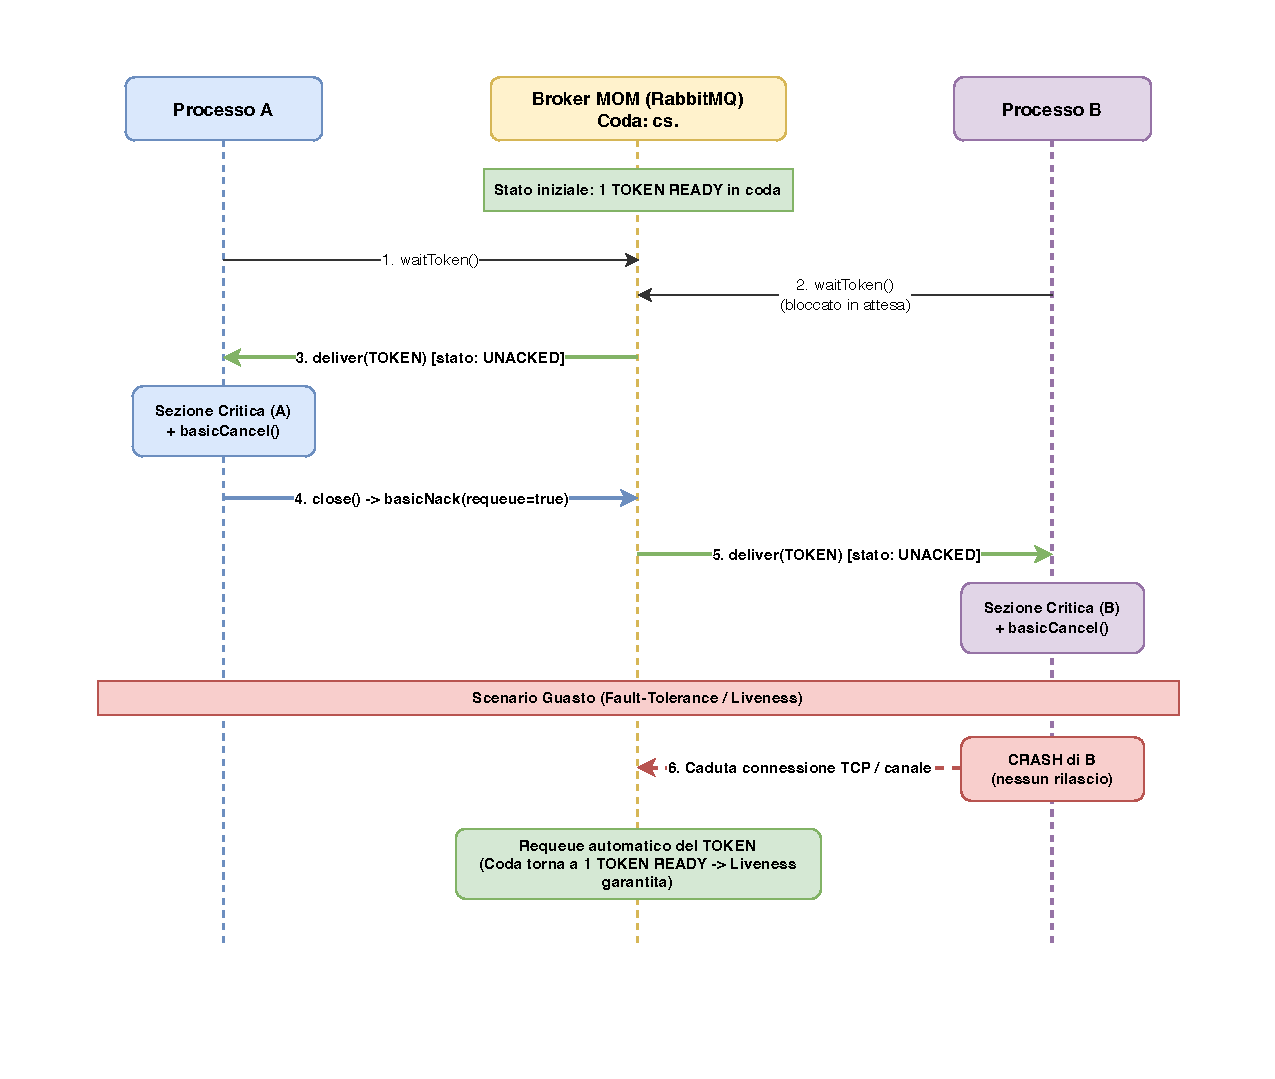
\includegraphics[width=\linewidth]{images/sezionecriticaconfailure.pdf}
    \caption{Flusso di acquisizione, rilascio e recupero automatico del token in caso di crash.}
    \label{fig:cs-token-flow}
\end{figure}

\section{Dettagli Implementativi e Casi Limite}
\subsection{Api utente}
E' stata sviluppada una libreria che espone tramite il meccanismo dell'\texttt{AutoCloseable} le primitive per inizializzare il servizio e per accedere a una critical section:

\noindent\begin{minipage}{\linewidth}
\begin{lstlisting}[language=Java, basicstyle=\ttfamily\small, frame=single, breaklines=true]
// 1. Bootstrap (eseguito una sola volta all'avvio del sistema)
CriticalSection.initialize("localhost", "cs.shared-resource");

// 2. Utilizzo da parte di un processo applicativo
try (CriticalSection cs = new CriticalSection("localhost", "cs.shared-resource")) {

    try (CriticalSection.CriticalHandler lock = cs.waitToken()) {
        // Codice eseguito in mutua esclusione distribuita
    } // Rilascio automatico del token

} // Chiusura automatica di canale e connessione AMQP
\end{lstlisting}\end{minipage}
Oppure in caso di un unico accesso all'interno di un programma
\begin{lstlisting}[language=Java, basicstyle=\ttfamily\small, frame=single, breaklines=true]

// Apertura della connession e accesso alla sezione critica in un unico comando
try (CriticalSection cs = new CriticalSection("localhost", "cs.shared-resource"); CriticalSection.CriticalHandler lock = cs.waitToken()) {
    // Sezione critica
}
\end{lstlisting}

\subsection{Il problema del Bootstrap}
RabbitMQ non fornisce nativamente un meccanismo per inizializzare una coda con un valore. E' stato deciso che questa deve essere un operazione fuori dal ciclo di vita applicativo del cliente e invece spostata nella fase di costruzione dell coda stessa. La libreria fornisce con \texttt{Initialize} la possibilità agli utilizzatori di inizializzare in maniera corretta una coda (ad esempio all'interno di una pipelin di CI/CD durante il setup di un servizio)

\subsection{Concorrenza intraprocesso}
La libreria è pensata in un ottica di programmazione distribuita non è stato quindi reputato necessario renderla thread safe. Igni istanza di \texttt{CriticalSection} è quindi progettata per essere utilizzata da un singolo thread.

\section{Testing e Verifica}
Per garantire test reali senza dipendere da Docker o da un'istanza esterna di RabbitMQ, si usa il broker AMQP 0-9-1 embedded in-memory tramite \textbf{Apache Qpid Broker-J}.

\begin{table}[h!]
\centering
\renewcommand{\arraystretch}{1.25}
\begin{tabular}{@{}>{\ttfamily\small} p{2.8cm} p{12cm}@{}}
\toprule
\normalfont\textbf{Proprietà} & \textbf{Scenario} \\
\midrule
Safety & 5 worker concorrenti su un contatore non sincronizzato con delay artificiale. Verifica mai più di uno in contemporanea e nessun aggiornamento perso. \\
Liveness (Crash) & Il Processo A acquisisce il token e chiude la connessione TCP senza rilasciare il handler. Verifica il requeue automatico e l'ingresso del Processo B. \\
Bootstrap & Verifica che una seconda chiamata a \texttt{initialize()} lanci \texttt{IllegalStateException}, impedendo la creazione di un doppio token. \\
API Locale & Verifica che un processo che detiene già il token non possa invocare nuovamente \texttt{waitToken()} sulla stessa istanza. \\
Liveness (Interrupt) & Un thread in attesa viene interrotto, verifica che al rilascio del detentore, un terzo processo entri senza deadlock. \\
\bottomrule
\end{tabular}
\caption{Riepilogo dei test di integrazione eseguiti su broker AMQP 0-9-1 embedded.}
\end{table}

\section{Limiti Noti e Possibili Estensioni}
\begin{itemize}
    \item \textbf{Partizioni di rete e pause GC (Split-Brain):} se un processo in sezione critica subisce una lunga pausa del Garbage Collector o una partizione di rete, il broker può chiudere la connessione per scadenza dell'heartbeat e riassegnare il token a un altro processo mentre il primo crede ancora di detenere il lock. In produzione questo scenario viene mitigato tramite l'utilizzo di GC moderni o tecniche come token incrementali.
    \item \textbf{Disponibilità del Broker:} il broker rappresenta un Single Point of Failure infrastrutturale.
\end{itemize}

\end{document}